\subsection{Misuratori hardware del consumo energetico}

I misuratori hardware del consumo energetico rappresentano l’approccio più diretto
per la misurazione dell’energia assorbita da un sistema di calcolo.
Tali soluzioni si basano su sensori fisici, esterni o integrati nell’hardware, e
forniscono misure caratterizzate da un’elevata accuratezza, in quanto l’energia viene
misurata direttamente a livello fisico.
Il monitoraggio può avvenire a livello di intera macchina o di specifici componenti
hardware, come CPU e memoria.

Una prima categoria è rappresentata dai misuratori hardware esterni, ovvero
dispositivi interposti fisicamente tra la sorgente di alimentazione e il sistema
sotto analisi.
Questi strumenti consentono di misurare l’energia realmente dissipata dall’intero
ecosistema hardware, includendo componenti spesso non osservabili tramite sensori
software, come gli alimentatori (PSU), i sistemi di raffreddamento e le perdite
resistive dei circuiti.
Per tale motivo, essi forniscono una visione completa del consumo energetico del
sistema.

Tuttavia, come ampiamente documentato in letteratura \cite{freina2024energysurvey}, l’adozione di misuratori
hardware esterni introduce una serie di criticità che ne limitano l’applicabilità in
contesti operativi su larga scala.
In primo luogo, la misurazione avviene tipicamente a livello di intero sistema
(\textit{full-system power}), rendendo complesso isolare il contributo energetico di
singoli componenti hardware o di specifiche entità software senza ricorrere a
strumentazione aggiuntiva e altamente invasiva.
In secondo luogo, l’integrazione di tali dispositivi in infrastrutture distribuite o
in ambienti di data center comporta costi economici e complessità operative
significative, legate sia all’acquisizione dell’hardware sia alla gestione del
cablaggio e della raccolta dei dati.

Per fornire un ordine di grandezza dell’investimento richiesto, nella Tabella
\ref{tab:costi_hardware} sono riportate alcune delle principali categorie di strumenti
utilizzati per il monitoraggio energetico hardware, insieme ai relativi ambiti di
applicazione.

\begin{table}[t]
\centering
\caption{Confronto tra principali tipologie di misuratori hardware esterni per il
monitoraggio del consumo energetico.}
\label{tab:costi_hardware}
\begin{tabular}{|l|p{4cm}|p{3cm}|p{4cm}|}
\hline
\textbf{Categoria} & \textbf{Esempio di Dispositivo} & \textbf{Costo Stimato} & \textbf{Ambito di utilizzo} \\ \hline
Entry-level &
TP-Link Kasa, Kill-A-Watt &
€30 -- €60 &
Analisi preliminari e misure indicative su singole workstation. \\ \hline
Enterprise &
APC Metered Rack PDU, Raritan PX &
€800 -- €2.500 &
Monitoraggio energetico di rack o gruppi di server in data center. \\ \hline
Laboratorio / R\&D &
Yokogawa WT310E, ZES ZIMMER LMG &
€2.500 -- €6.000+ &
Misurazioni ad alta precisione per validazione scientifica e ricerca accademica. \\ \hline
\end{tabular}
\end{table}

I dispositivi di fascia entry-level offrono generalmente frequenze di campionamento
limitate, dell’ordine di pochi Hertz, risultando adeguati per analisi preliminari su
singole macchine.
Al contrario, gli strumenti utilizzati in ambito di ricerca e validazione
scientifica consentono misurazioni ad alta frequenza e un’elevata precisione, a
fronte di costi significativamente più elevati.

Oltre ai misuratori hardware esterni, i moderni processori integrano sensori
energetici direttamente a livello di chip, rendendo possibile l’accesso a stime
del consumo energetico tramite interfacce software.
Un esempio significativo è rappresentato dalla tecnologia \textit{Running Average
Power Limit} (RAPL), introdotta da Intel, che consente di ottenere informazioni
sul consumo energetico di diversi domini di potenza interni al processore
\cite{intel-rapl, rapl_description}.

RAPL suddivide il consumo energetico del sistema in un insieme di domini logici,
ciascuno dei quali rappresenta una porzione specifica dell’hardware.
In particolare, il dominio \textit{Package} (PKG) rappresenta il consumo energetico
complessivo del processore, includendo i core, le cache e le interconnessioni interne.
Il dominio \textit{Power Plane 0} (PP0) è invece associato principalmente ai core
di calcolo della CPU, mentre altri domini, come \textit{DRAM}, forniscono una stima
del consumo energetico della memoria principale, quando supportati
dall’architettura.

La Figura~\ref{fig:rapl-domains} illustra un esempio di suddivisione del consumo
energetico secondo il modello RAPL, evidenziando come i diversi domini di potenza
corrispondano a specifiche componenti hardware del sistema.
Questa rappresentazione consente di comprendere come le misure fornite da RAPL
siano intrinsecamente legate all’organizzazione fisica del processore e non alle
singole entità software in esecuzione.

\begin{figure}[t]
    \centering
    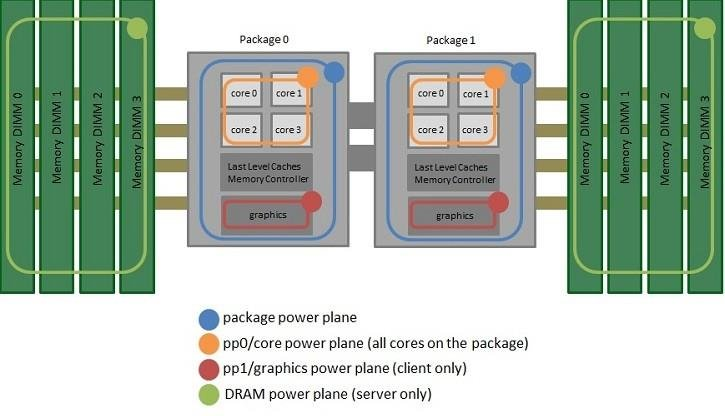
\includegraphics[width=0.8\textwidth]{figures/RAPL-Power-Domains-1.png.jpeg}
    \caption{Esempio di domini di potenza definiti dal modello RAPL. Il dominio
    \textit{Package} rappresenta il consumo energetico complessivo della CPU,
    mentre domini più specifici, come \textit{PP0} e \textit{DRAM}, forniscono
    stime riferite rispettivamente ai core di calcolo e alla memoria principale.}
    \label{fig:rapl-domains}
\end{figure}

Il funzionamento di RAPL si basa su modelli energetici interni al processore,
calibrati dal produttore, che stimano l’energia consumata a partire da eventi
hardware e contatori interni.
Sebbene tali misure non rappresentino una misurazione fisica diretta dell’energia,
diversi studi hanno dimostrato come esse offrano un buon compromesso tra accuratezza
e semplicità di utilizzo, risultando particolarmente adatte al monitoraggio
energetico a runtime\cite{rapl-evaluation}.
Le informazioni rese disponibili da RAPL possono essere lette tramite interfacce
standard del sistema operativo, consentendo la loro integrazione in strumenti di
monitoraggio software.

Nonostante questi vantaggi, i sensori hardware integrati presentano limiti
strutturali quando applicati a contesti software moderni.
La granularità delle misure è tipicamente limitata al livello di macchina o di
componente hardware e non consente di attribuire in modo diretto il consumo
energetico alle singole applicazioni, ai container o alle singole invocazioni.
In ambienti multi-tenant e containerizzati, come quelli tipici del Serverless
Computing, il consumo energetico osservato è quindi il risultato dell’esecuzione
concorrente di più entità software, rendendo complessa l’analisi del comportamento
energetico delle singole funzioni.

Inoltre, le misure fornite da RAPL sono di natura cumulativa e non distinguono in
modo esplicito tra le diverse fasi di esecuzione, quali inizializzazione,
esecuzione vera e propria e periodi di inattività.
Questo aspetto risulta particolarmente critico nel Serverless Computing, dove
fenomeni come il cold start e il riutilizzo dei container hanno un impatto
significativo sul consumo energetico complessivo.
Di conseguenza, pur costituendo una base affidabile per la stima dell’energia a
livello di sistema, i sensori hardware integrati non risultano sufficienti per
supportare analisi a grana fine e decisioni di gestione energetica a livello
software.


Alla luce di queste considerazioni, sebbene i misuratori hardware costituiscano una base affidabile per la misurazione dell’energia, essi risultano insufficienti per
supportare il monitoraggio continuo e a grana fine richiesto da ambienti dinamici e
distribuiti.
In tali contesti emerge la necessità di soluzioni in grado di offrire una maggiore
flessibilità e di integrarsi in modo più stretto con i meccanismi di esecuzione del
software.

